\section{Results}
\subsection{Main results}
PR-LFL reaches client-macro NLL 0.645/0.188 (0.6446/0.1880 before rounding) and accuracy 75.57\%/92.97\% on CIFAR-10/FashionMNIST. Changing the center gives NLL gains of 0.0358/0.0182 and accuracy gains of 0.1777/0.1730 percentage points (Table~\ref{tab:main}). Learned correction reduces NLL over fixed prior addition by 0.0282/0.0222, placing the prior inside a fitted predictor.

At a matched budget (54,067 B for uniform3, 54,808 B for TopK), a TopK compressor reaches NLL 0.670 and a FedRoD-linear reference 0.677 on CIFAR-10, against 0.645 for uniform3 with the prior center; both are matched in-house implementations over the same three paired seeds. Table~\ref{tab:main} shows that the correction also holds under dense FedAvg and FedProx.\par\vspace{-\baselineskip}
\begin{table}[!htb]
\centering\small
\setlength{\tabcolsep}{5pt}
\caption{Prior centering lowers NLL on both tasks and under two dense shared-training paths. Dense FedAvg/FedProx are matched in-house implementations trained on the same partitions and seeds. Client-macro accuracy (\%) / NLL, three-seed mean $\pm$ sample SD.}\label{tab:main}
\begin{tabular}{lrrrr}\toprule
& \multicolumn{2}{c}{CIFAR-10} & \multicolumn{2}{c}{FashionMNIST}\\
Predictor & Acc. (\%) & NLL & Acc. (\%) & NLL\\\midrule
Shared model & $38.96\pm0.77$ & $1.677\pm0.029$ & $69.79\pm1.69$ & $0.749\pm0.035$\\
Shared + prior & $74.60\pm0.82$ & $0.673\pm0.014$ & $91.97\pm0.29$ & $0.210\pm0.011$\\
Zero vector (20d) & $75.39\pm0.68$ & $0.680\pm0.014$ & $92.80\pm0.37$ & $0.206\pm0.012$\\
Prior BCTS (11d) & $75.56\pm0.52$ & $0.646\pm0.013$ & $92.84\pm0.38$ & $0.192\pm0.011$\\
Prior vector (20d) & $75.57\pm0.60$ & $0.645\pm0.014$ & $92.97\pm0.44$ & $0.188\pm0.011$\\
FedAvg + zero & $75.62\pm0.52$ & $0.679\pm0.013$ & $92.69\pm0.41$ & $0.205\pm0.013$\\
FedProx + zero & $75.03\pm0.41$ & $0.691\pm0.013$ & $92.62\pm0.26$ & $0.208\pm0.013$\\
FedAvg + prior & $75.58\pm0.54$ & $0.644\pm0.012$ & $92.94\pm0.41$ & $0.187\pm0.011$\\
FedProx + prior & $74.96\pm0.59$ & $0.655\pm0.013$ & $92.84\pm0.35$ & $0.189\pm0.011$\\
Local Linear (650d) & $74.10\pm0.34$ & $0.725\pm0.019$ & $92.22\pm0.46$ & $0.226\pm0.018$\\
\bottomrule
\end{tabular}
\end{table}


\begin{table}[!htb]\centering\small\setlength{\tabcolsep}{2.2pt}
\caption{Prior-centered vector scaling lowers NLL and Brier score; BCTS gives lower client ECE. Upper: Brier/ECE (lower is better), ECE in percentage points. P denotes prior centering. Lower: means; accuracy is a proportion.}\label{tab:quality}
\begin{tabular}{@{}lrrr@{\hspace{3.7pt}}rrr@{}}\toprule
& \multicolumn{3}{c}{CIFAR-10} & \multicolumn{3}{c}{FashionMNIST}\\
Predictor & Brier & ECE$_c$ & ECE$_p$ & Brier & ECE$_c$ & ECE$_p$\\\midrule
Zero & $0.343\pm0.008$ & $6.15\pm0.20$ & $1.35\pm0.41$ & $0.108\pm0.006$ & $3.69\pm0.45$ & $0.58\pm0.20$\\
P-BCTS & $0.341\pm0.007$ & $5.37\pm0.23$ & $1.30\pm0.10$ & $0.105\pm0.005$ & $2.82\pm0.07$ & $0.45\pm0.21$\\
P-vector & $0.340\pm0.008$ & $5.48\pm0.17$ & $1.49\pm0.24$ & $0.103\pm0.006$ & $3.05\pm0.18$ & $0.47\pm0.20$\\\bottomrule
\end{tabular}
\par\medskip
\begin{tabular}{lrrrr}\toprule
& \multicolumn{2}{c}{CIFAR-10} & \multicolumn{2}{c}{FashionMNIST}\\
Endpoint & Zero & Prior & Zero & Prior\\\midrule
Weighted NLL & 0.6788 & 0.6571 & 0.1588 & 0.1486\\
Weighted accuracy & 0.7475 & 0.7471 & 0.9462 & 0.9473\\
Client accuracy $q_{10}$ & 0.6027 & 0.6065 & 0.8578 & 0.8566\\\bottomrule
\end{tabular}
\end{table}

The prior vector lowers mean NLL and Brier score, whereas same-prior BCTS gives lower mean client ECE (Table~\ref{tab:quality}). Weighted NLL falls by 0.0217/0.0102, compared with the larger client-macro gains, motivating a closer look at how benefit varies across heterogeneous clients.

\subsection{Heterogeneity sweep}
In this three-point sweep, mean gain increases as heterogeneity strengthens (Fig.~\ref{fig:heterogeneity}a). As $\alpha$ decreases from 1.0 through 0.5 to 0.1, gain rises from 0.0042 through 0.0101 to 0.0408 on CIFAR-10 and from 0.0024 through 0.0047 to 0.0132 on FashionMNIST. Each $\alpha$ uses one partition realization and three model seeds. At $\alpha=0.1$, development NLL improves in 60/60 CIFAR and 59/60 Fashion client--seed pairs, concentrating the largest mean benefit at the strongest heterogeneity measured in this sweep.

\begin{figure}[!htb]\centering
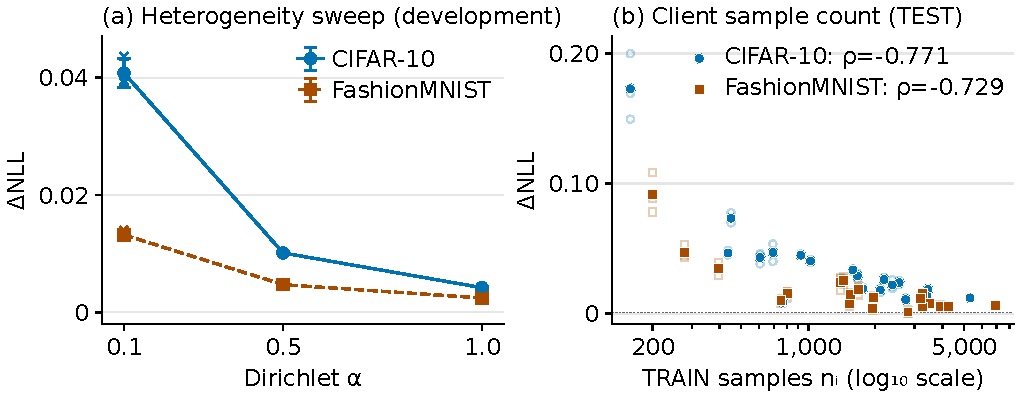
\includegraphics[width=0.8\linewidth]{figures/figure2_heterogeneity_dual.pdf}
\caption{Mean gain is larger under stronger heterogeneity across the three-point sweep. (a) Development gain versus $\alpha$: three-seed means, sample SD and seed markers. (b) Saved TEST gain versus client TRAIN sample count $n_i$ (log axis): twenty client means per task and seed observations. Positive $\Delta\mathrm{NLL}=\mathrm{NLL}(\mathrm{zero})-\mathrm{NLL}(\mathrm{prior})$ favors prior centering.}\label{fig:heterogeneity}
\end{figure}

\subsection{Who benefits: client sample count}
Gain is negatively associated with client TRAIN sample count, with Spearman $\rho=-0.771/-0.729$ on CIFAR-10/FashionMNIST (Fig.~\ref{fig:heterogeneity}b). Each client mean averages three seeds within the original fixed partition. This association places the measured gain among smaller clients, where the mean-loss penalty $\lambda/|D_i|$ gives the prior center greater weight.

\subsection{Class-alignment control}
Permuting class labels in the prior raises development NLL by 0.071/0.044 on CIFAR-10/FashionMNIST at fixed center norm and predictor capacity, attributing the benefit to class alignment.
